\chapter{Resultados Experimentais }
\label{cap:resultados}

\section{Resultados}

\subsection{Divisão dos dados entre treino e validação}

\begin{figure}[H]
  \centering
  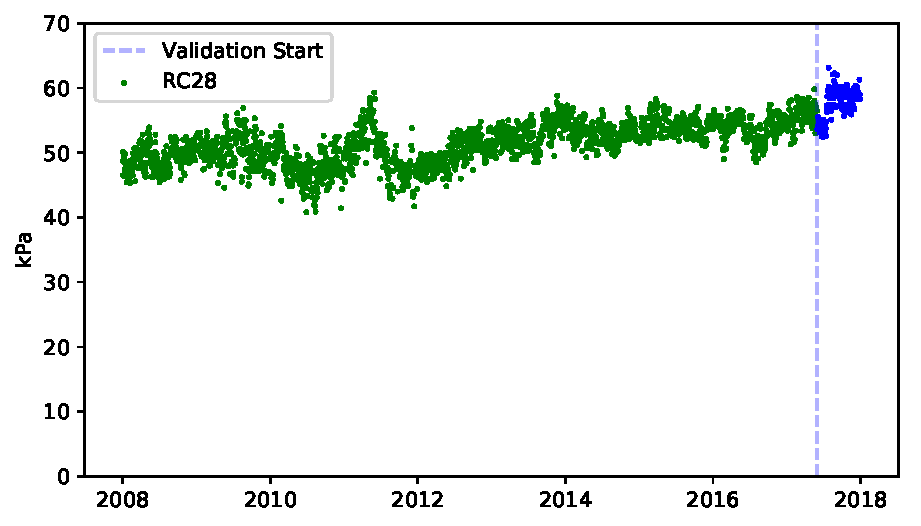
\includegraphics[width=0.9\columnwidth]{train_dev.pdf}
  \caption{Divisão do dataset para a saída RC28, os pontos verdes foram usados para
    treino e os pontos azuis usados para validação.}
  \label{fig:divrc28}
\end{figure}

\subsection{Abordagem Não-Temporal}

Modelos de Aprendizagem Automática não-temporais foram usados para treinar e validar os dados, para esses modelos usamos a biblioteca Sklearn.
As avaliações de RMSE de todo o conjunto de validação estão apresentados por modelos na Imagem~\ref{fig:linmodels}  

\begin{figure}[H]
  \centering
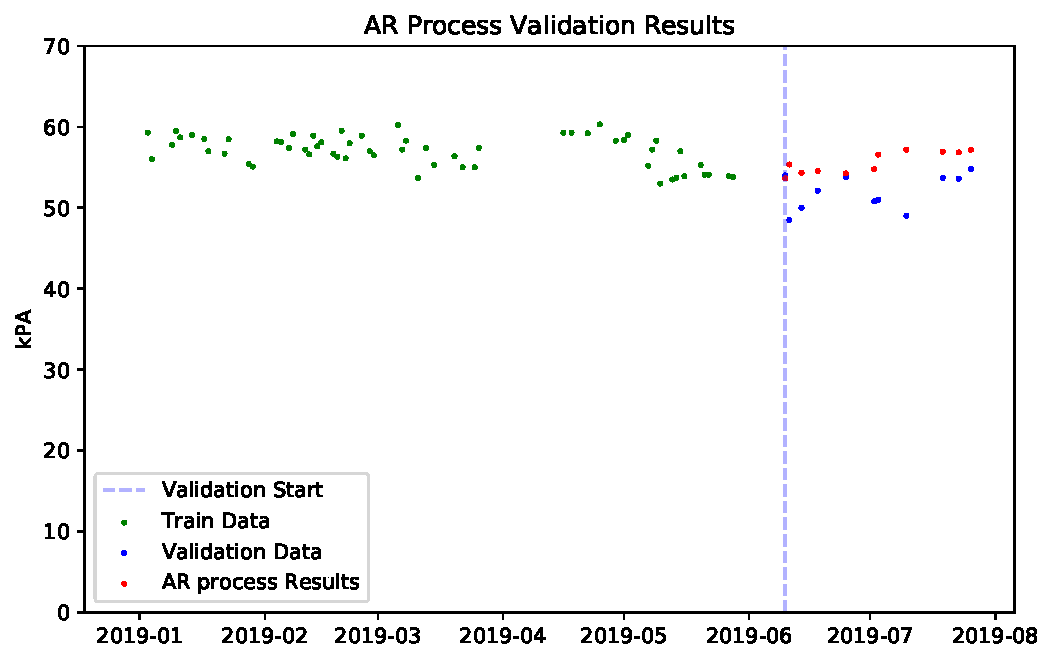
\includegraphics[width=0.9\columnwidth]{linear_exp.pdf}
\caption{Predições nos dados de validação nos experimentos com modelos não-temporais. }
\label{fig:linmodels}
\end{figure}

Na Tabela~\ref{tb:rmse_lin} reportamos os erros para predições imediatamente
após o fim do último dia de dados usados para treino. Iremos mostrar o
erro para o dia seguinte, três dias depois e então uma semana após o último dia
de dados usados para treinamento.

\begin{center}
\begin{table}[htbp]
\caption{RMSE values by forecast span}
\centering
\begin{tabular}{rr}
\hline
 Regressão Linear & RMSE\\
\hline
24h & 2.94\\
3d & 0.13\\
7d & 5.43\\
\hline
Rede Neural & RMSE\\
\hline
24h & 3.70\\
3d & 1.26\\
7d & 6.04\\
\hline
Random Forest & RMSE\\
\hline
24h & 1.61\\
3d & 1.36\\
7d & 5.83\\
\end{tabular}

\label{tb:rmse_lin}
\end{table}
\end{center}

 Reportamos distribuição dos valores previstos, até 1 mês após a data
onde começam os dados de validação (i.e. os dados não usamos para treinamento), a Imagem \ref{fig:distr_lin} permite comparar as distribuições previstas pelos 3 modelos:

\begin{figure}[H]
\label{fig:distr_lin}
\centering
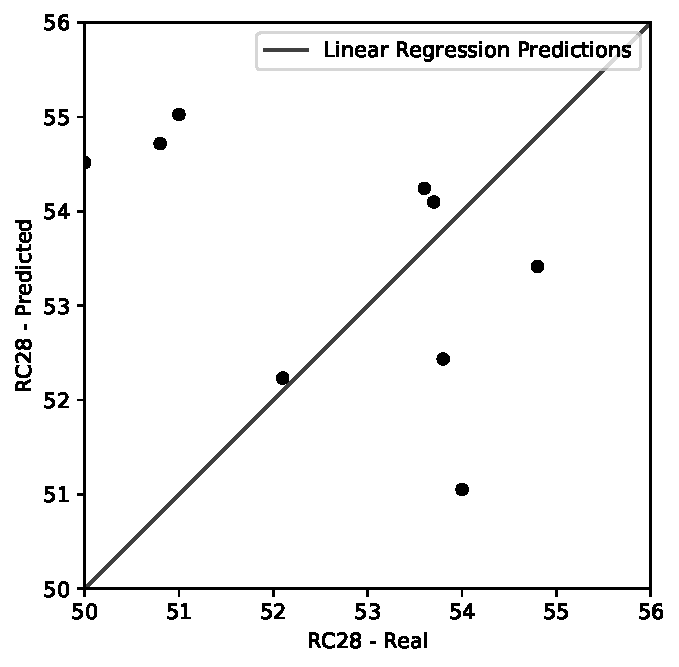
\includegraphics[width=.3\textwidth]{qq-LinearRegression.pdf} \hfill
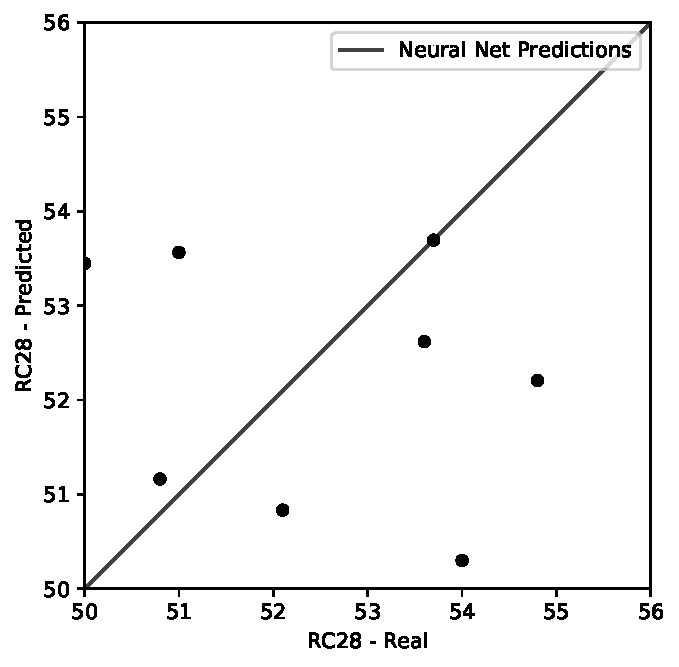
\includegraphics[width=.3\textwidth]{qq-NeuralNet.pdf} \hfill
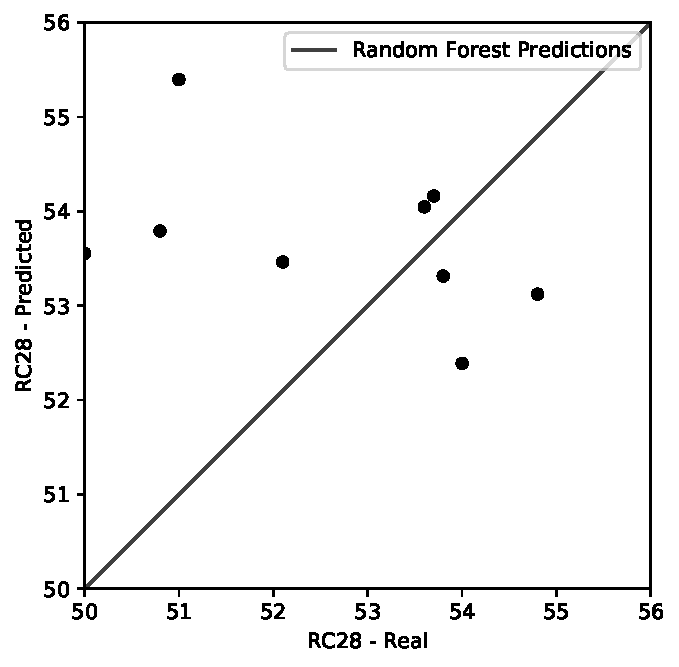
\includegraphics[width=.3\textwidth]{qq-RandomForest.pdf} 
\caption{Valores reais plotados contra os valores previstos para análise da distribuição aprendida por cada modelo} 
\end{figure}

Para modelagem de séries temporais, é comum se estudar o resíduo das
predições. É assumido em uma tarefa de regressão que o resíduo é distribuído
normalmente e com média zero.

\begin{figure}[H]
  \label{fig:res_lin}
  \centering
  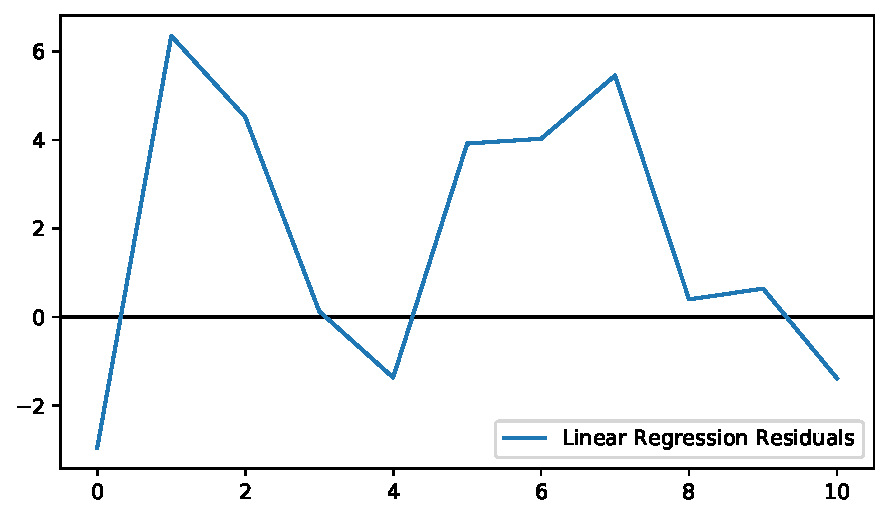
\includegraphics[width=.3\textwidth]{residuals-LinearRegression.pdf} \hfill
  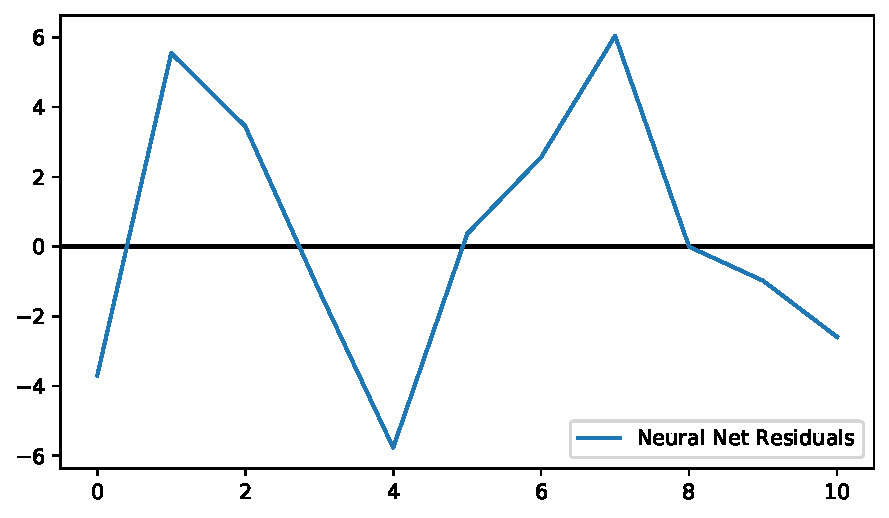
\includegraphics[width=.3\textwidth]{residuals-NeuralNet.pdf} \hfill
  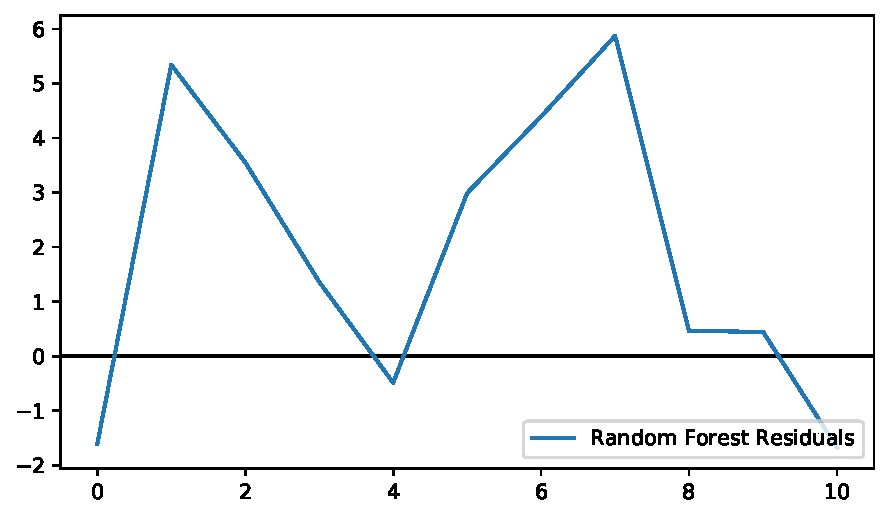
\includegraphics[width=.3\textwidth]{residuals-RandomForest.pdf} 
  \caption{Distribuição dos Erros de cada modelo. Como esperado, todos os erros flutuam em torno da média 0. } 
\end{figure}

\subsection{Regressão Linear Dinâmica com Filtragem Exponencial}

Para efeito de comparação de resultados, iremos aplicar o método proposto em
\citep{grecialin}. Primeiramente apresentamos a variação do erro de treino em
função do parâmetro $t_d$ i.e. o tamanho do conjunto de treino para cada
regressão. Apresentamos os resultados com e sem a aplicação da filtragem
proposta no trabalho \citep{grecialin}.

\begin{figure}[H]
  \centering
  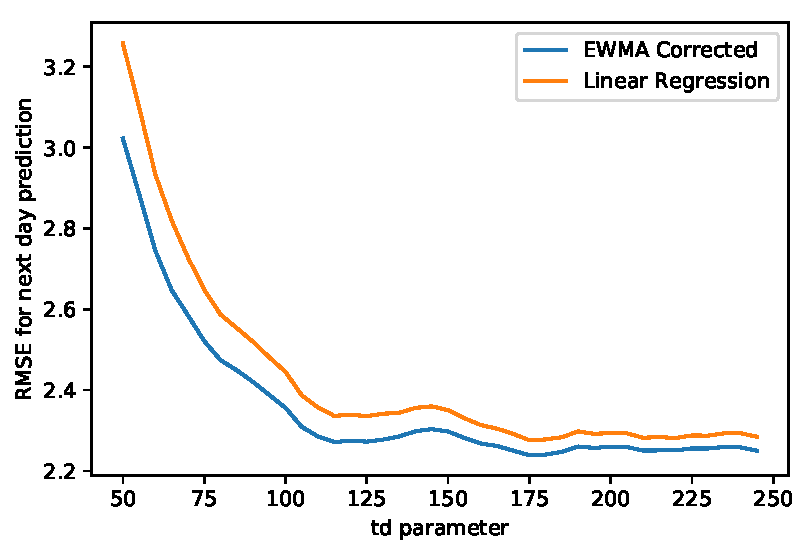
\includegraphics[width=0.9\columnwidth]{tdparameter.pdf}
  \caption{Erro de treino em função do parâmetro $t_d$}
  \label{fig:tdparam}
\end{figure}

Os resultados do modelo em todo o período de validação, bem como o erro são
reportados a seguir:

\begin{figure}[H]
  \centering
  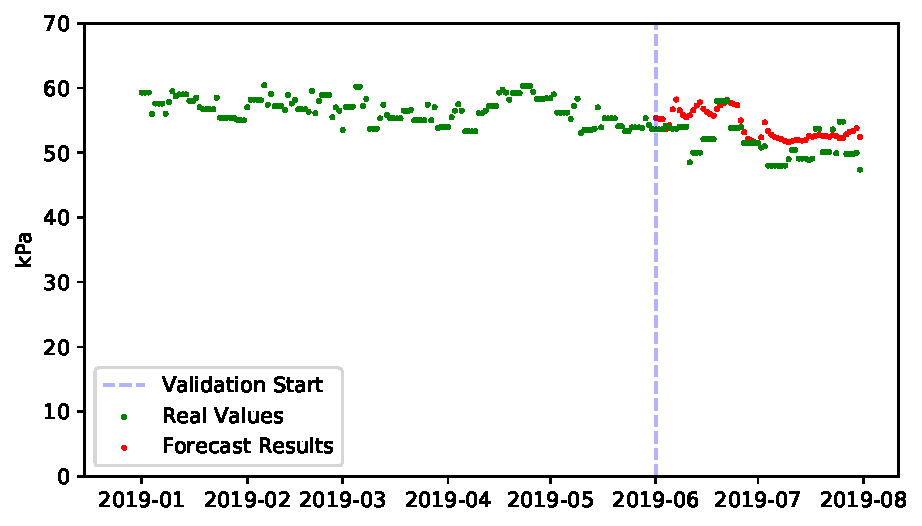
\includegraphics[width=0.9\columnwidth]{forecast_lin_reg_win.pdf}
  \caption{Predições no conjunto de validação do modelo de regressão linear dinâmico}
  \label{fig:tdparam}
\end{figure}

\begin{center}
  \begin{table}[htbp]
    \caption{RMSE values by forecast span}
    \centering
    \begin{tabular}{rr}
      \hline
      Reg. Linear com Filtragem Exponencial & RMSE\\
      \hline
      24h & 1.79 \\ 
      3d & 1.47\\
      7d & 2.36\\
    \end{tabular}

    \label{tb:rmse_exp}
  \end{table}
\end{center}
São reportadas também a distribuição das predições e dos resíduos do modelo exponencial.

\begin{figure}[H]
  \label{fig:distr_exp}
  \centering
  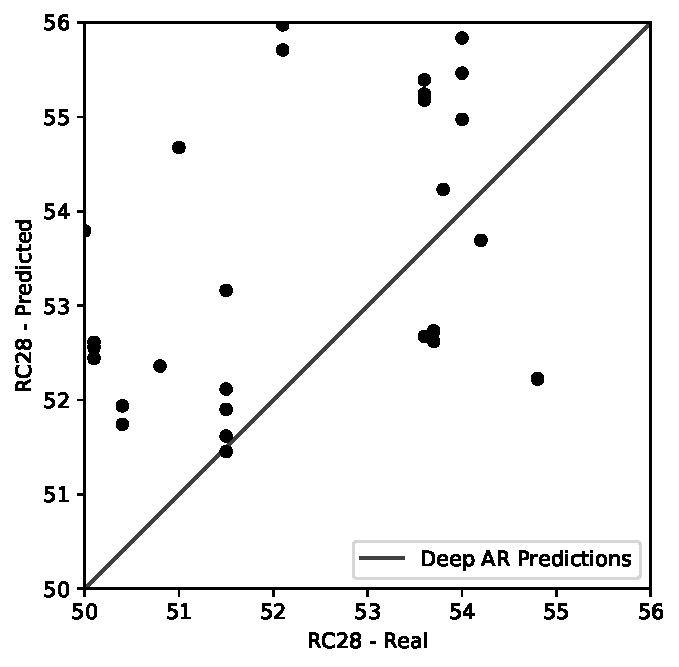
\includegraphics[width=.5\textwidth]{qq_forecast_lin_reg_win.pdf} \hfill
  \caption{Valores reais plotados contra os valores previstos para análise da
    distribuição aprendida pelo modelo exponencial} 
\end{figure}


\begin{figure}[H]
  \label{fig:res_exp}
  \centering
  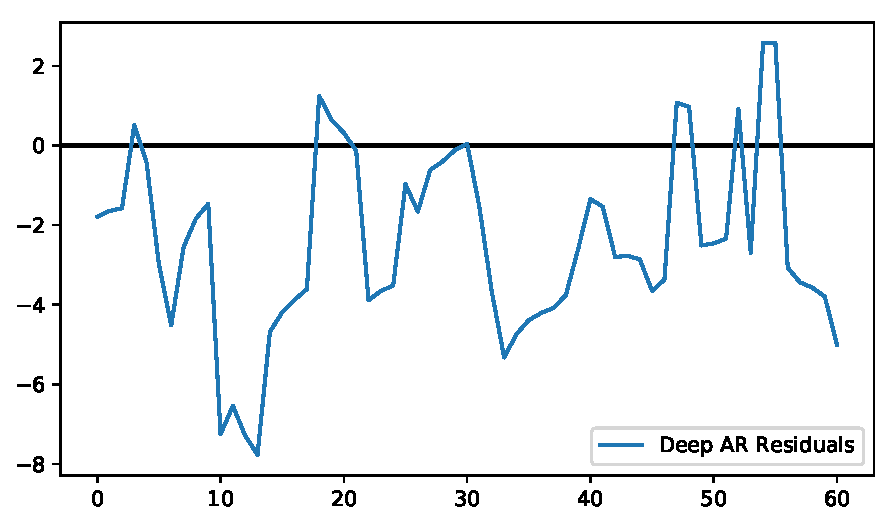
\includegraphics[width=.5\textwidth]{res_forecast_lin_reg_win.pdf} \hfill
  \caption{Distribuição dos resíduos do modelo exponencial} 
\end{figure}

\subsection{Modelos Bayesianos para Séries Temporais}


Todos os modelos foram implementados usando a biblioteca Pytorch \cite{pytorch}, para os Processos Gaussianos usamos a biblioteca GPyTorch \cite{gpytorch}. As tuplas de treino são da forma $(RC28_{t},\{\})$. 

Para os modelos DeepAR e Encoder-Decoder-Forecaster, as predições começam após
uma janela inteira de dias ser codificada pelas redes Encoder.
Apenas então os modelos terão informação para gerar predições. O Modelo Deep
Factors não necessita de uma janela pois sua arquitetura permite e emissão de
predições imediatamente após o primeiro timestep ser recebido,
e o Processo Gaussiano gera incertezas para todo o dataset de validação ao mesmo tempo, visto que é uma operação matricial. \\

Na Tabela~\ref{tb:rmse} reportamos os erros para predições imediatamente no
começo após o fim do último dia de dados usados para treino. Iremos mostrar o
erro para o dia seguinte, três dias depois e então uma semana após o último dia
de dados usados para treinamento.

\begin{center}
\begin{table}[htbp]
\caption{RMSE values by forecast span}
\centering
\begin{tabular}{rr}
\hline
Deep Factors & RMSE\\
\hline
24h & 0.18\\
3d & 2.36\\
7d & 1.83\\
\hline
Deep AR & RMSE\\
\hline
24h & 0.07\\
3d & 1.37\\
7d & 1.44\\
\hline
Encoder Decoder & RMSE\\
\hline
24h & 0.06\\
3d & 0.44\\
7d & 0.80\\
\end{tabular}

\label{tb:rmse}
\end{table}
\end{center}

A Imagem \ref{fig:distr} compara as distribuições previstas para o mês
de dados de validação pelos 3 modelos:

\begin{figure}[H]
\centering
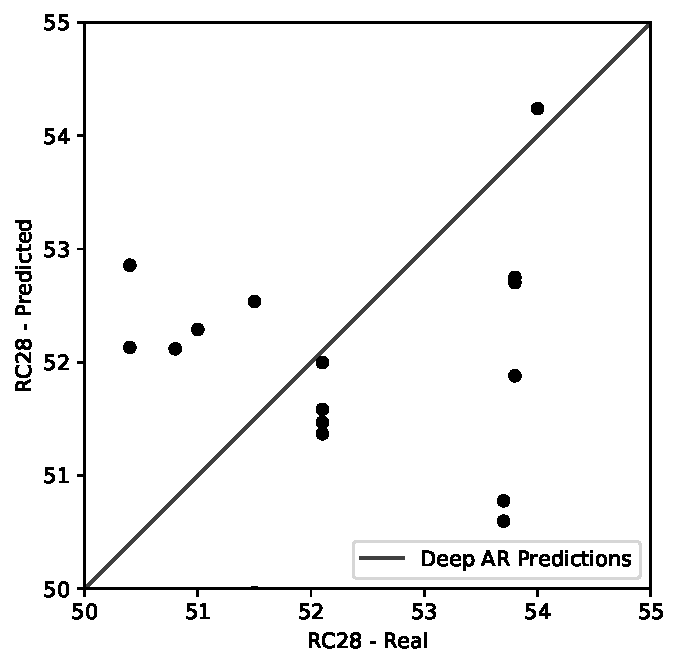
\includegraphics[width=.3\textwidth]{qq_deep_ar.pdf} \hfill
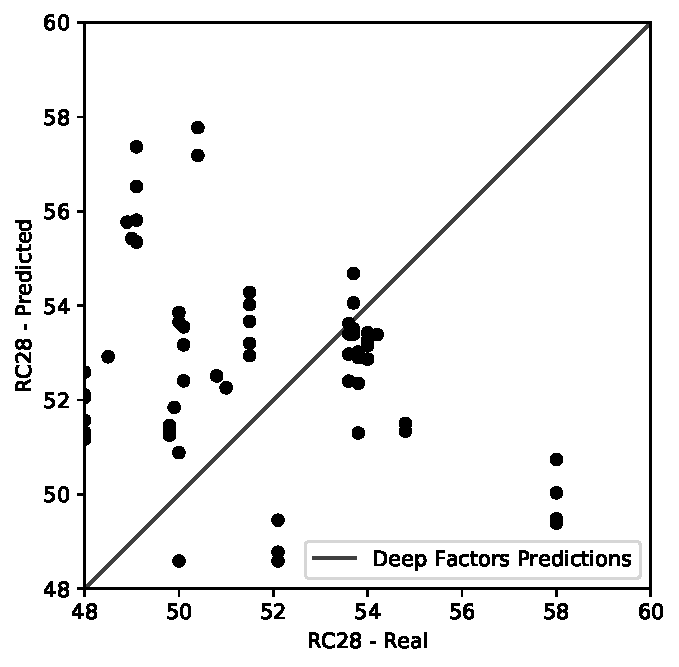
\includegraphics[width=.3\textwidth]{qq_deep_factors.pdf} \hfill
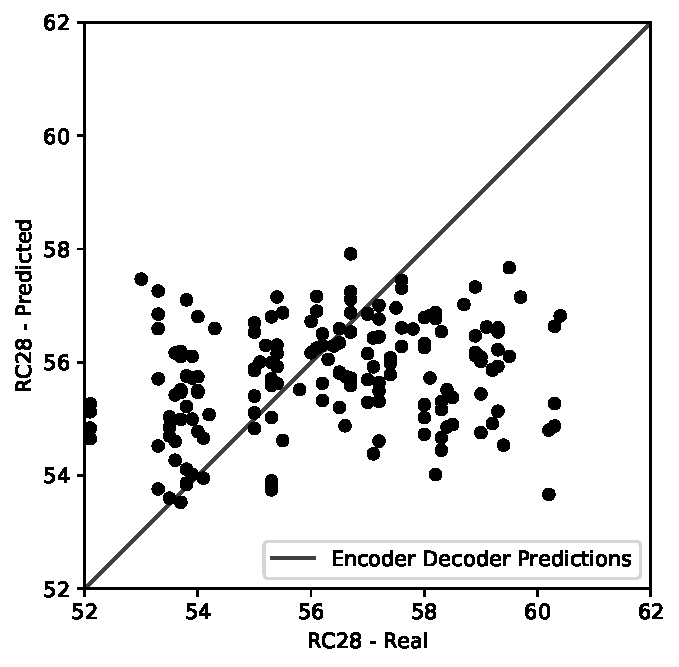
\includegraphics[width=.3\textwidth]{qq_enc_dec.pdf} 
\caption{Valores reais plotados contra os valores previstos para análise da distribuição aprendida por cada modelo} 
\label{fig:distr}
\end{figure}


Finalmente, os valores e incertezas previstos pelos modelos:


\begin{figure}[H]
  \label{fig:fordeepar}
  \centering
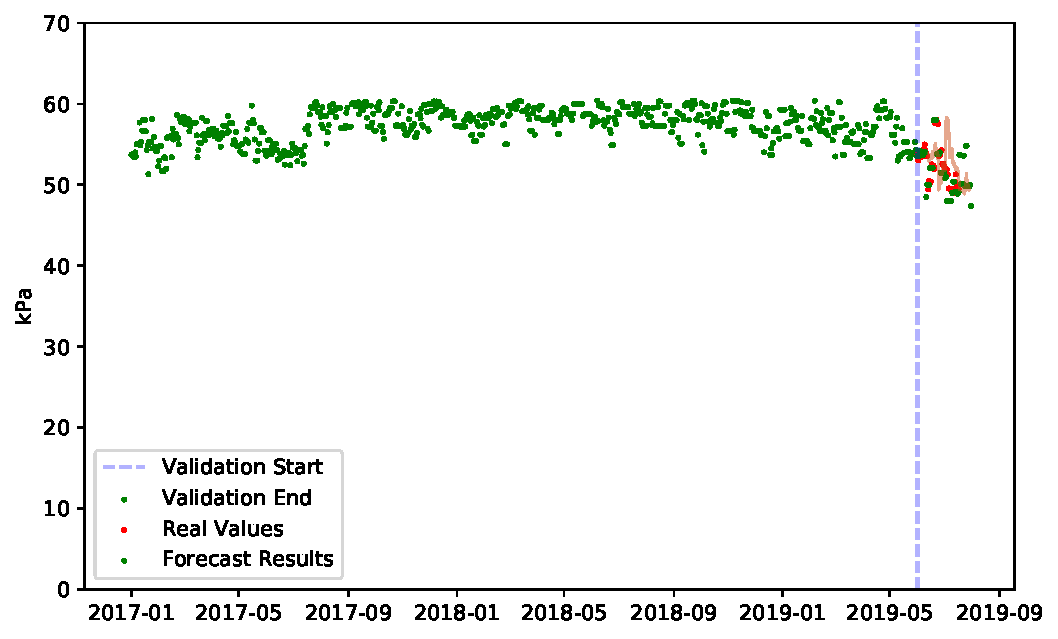
\includegraphics[height=.3\textwidth]{forecast_deep_ar.pdf} 
\caption{Predição para todos os dados de validação para o modelo Deep AR}
\end{figure}

\begin{figure}[H]
  \label{fig:fordeepfactors}
  \centering
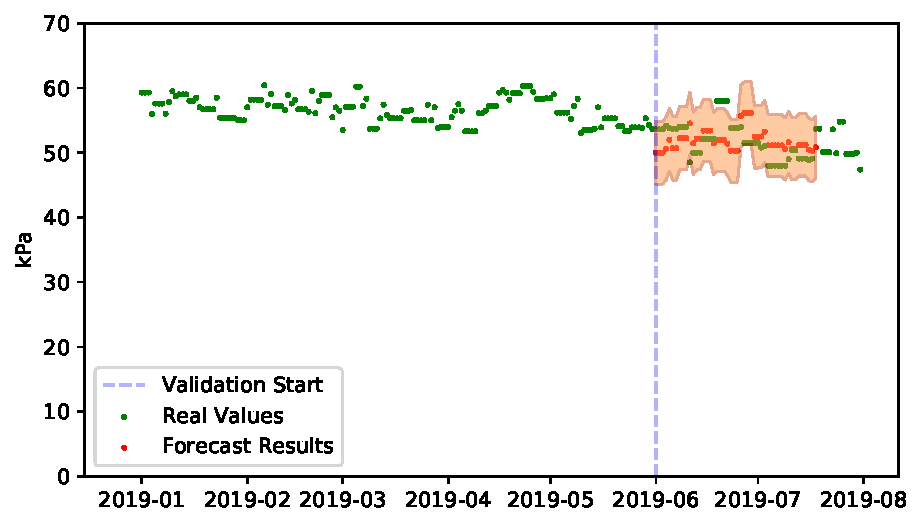
\includegraphics[height=.3\textwidth]{forecast_deep_factors.pdf} 
\caption{Predição para todos os dados de validação para o modelo Deep Factors}
\end{figure}

\begin{figure}[H]
  \label{fig:forencdec}
  \centering
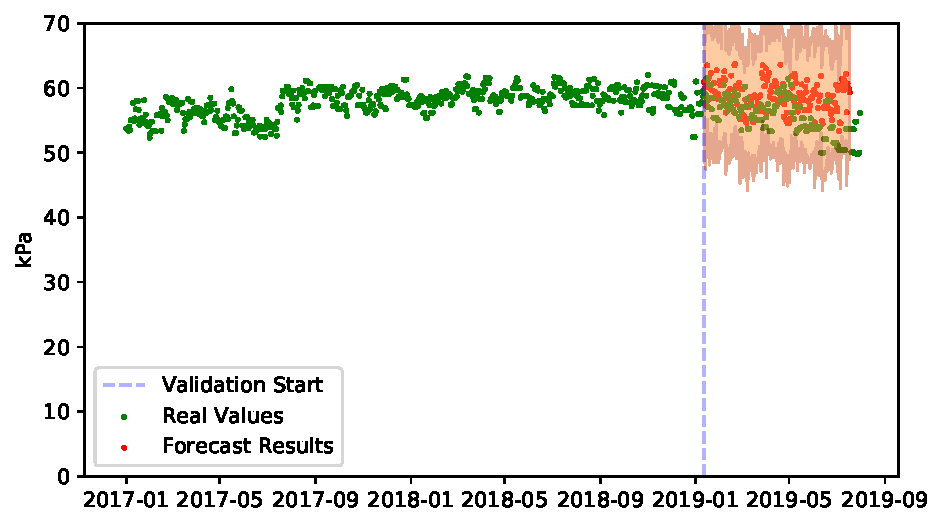
\includegraphics[height=.3\textwidth]{forecast_enc_dec.pdf} 
\caption{Predição para todos os dados de validação para o modelo Encoder Decoder Forecaster} 
\end{figure}


Para modelagem de séries temporais, é também comum estudarmos o resíduo das
predições. É assumido em uma tarefa de regressão que o resíduo é distribuído
normalmente com média zero.


\begin{figure}[H]
\label{fig:res}
\centering
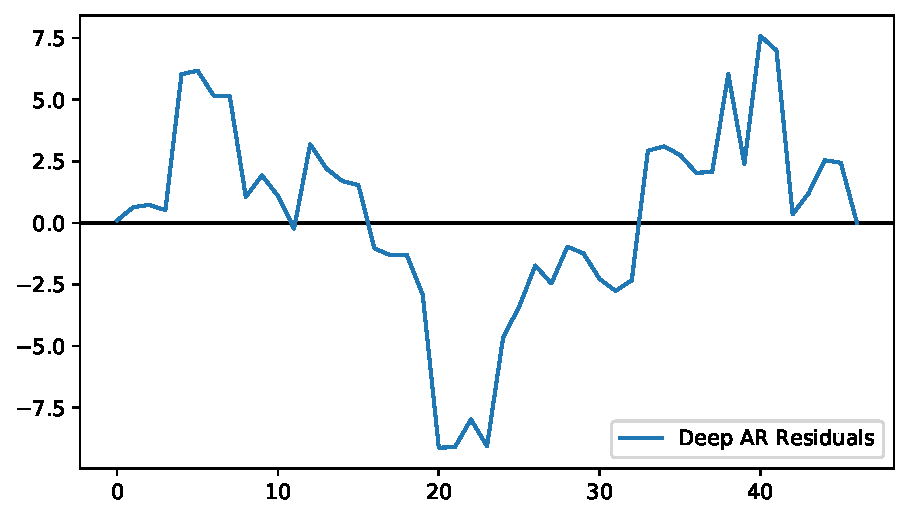
\includegraphics[width=.3\textwidth]{res_deep_ar.pdf} \hfill
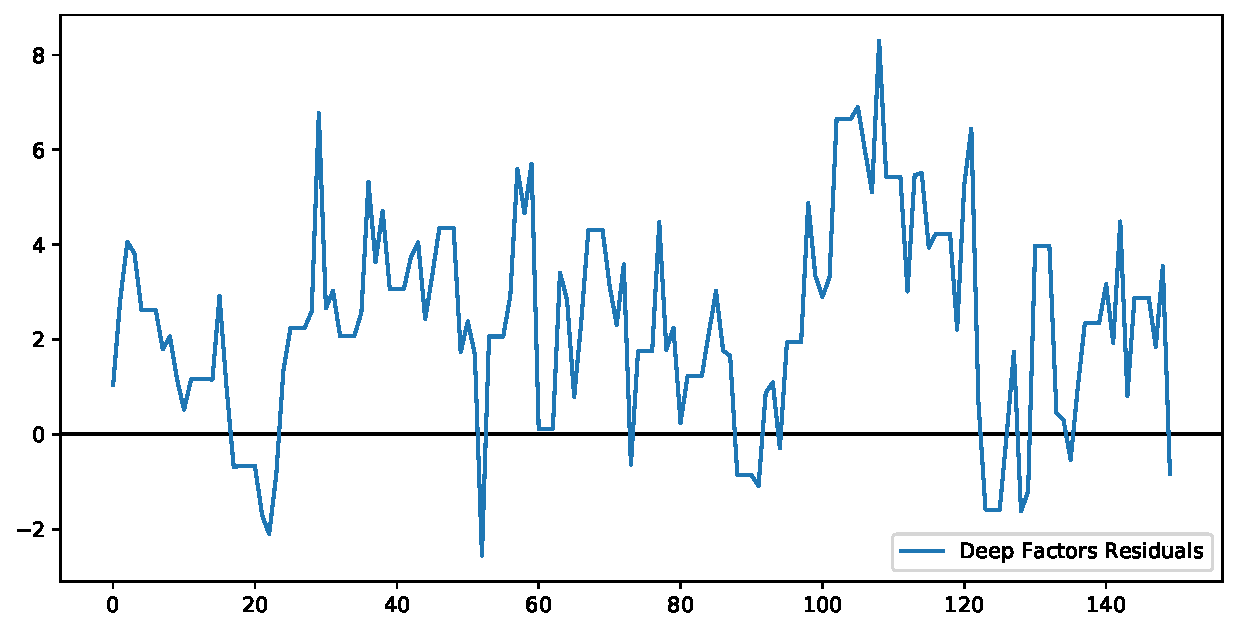
\includegraphics[width=.3\textwidth]{res_deep_factors.pdf} \hfill
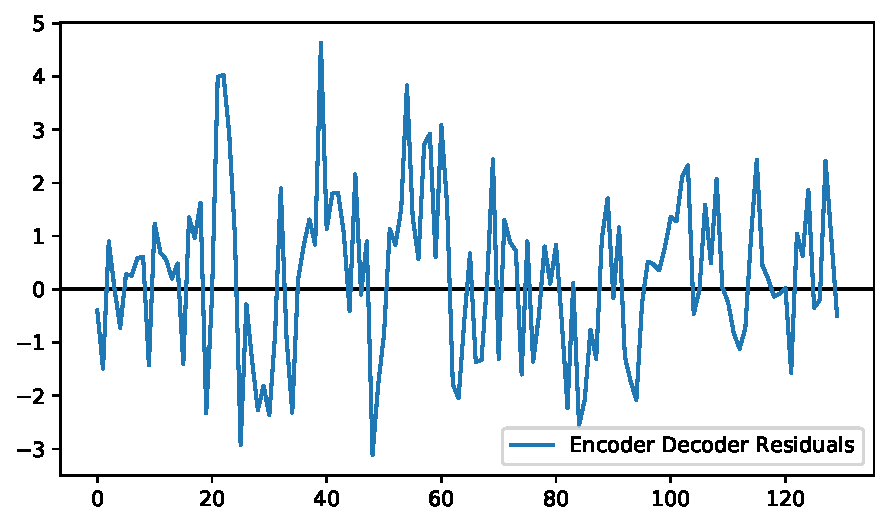
\includegraphics[width=.3\textwidth]{res_enc_dec.pdf} 
\caption{Distribuição dos Erros de cada modelo. Como esperado, todos os erros flutuam em torno da média 0. } 
\end{figure}




Os modelos de DL obtiveram um erro menor na predição do dia seguinte bem como em
horizontes próximos de tempo, tanto em relação aos modelos não-temporais como em
relação ao modelo filtrado expoencialmente.


% Local Variables:
% TeX-master: "../quali"
% End:
